\documentclass[twocolumn,a4j]{jsarticle}
\setlength{\topmargin}{-20.4cm}
\setlength{\oddsidemargin}{-10.4mm}
\setlength{\evensidemargin}{-10.4mm}
\setlength{\textwidth}{18cm}
\setlength{\textheight}{26cm}

\usepackage[top=15truemm,bottom=20truemm,left=20truemm,right=20truemm]{geometry}
\usepackage[latin1]{inputenc}
\usepackage{amsmath}
\usepackage{amsfonts}
\usepackage{amssymb}
\usepackage[dvipdfmx]{graphicx}
\usepackage[hang,small,bf]{caption}
\usepackage[subrefformat=parens]{subcaption}
\usepackage[dvipdfmx]{color}
\usepackage{listings}
\usepackage{listings,jvlisting}
\usepackage{geometry}
\usepackage{framed}
\usepackage[dvipdfmx]{hyperref}
\usepackage{ascmac}
\usepackage{enumerate}
\usepackage{tabularx}
\usepackage{cancel}
\usepackage{scalefnt}
\usepackage{overcite}
\usepackage{otf}
\usepackage{multicol}
\usepackage[geometry]{ifsym}
\usepackage{array}

\renewcommand{\figurename}{Fig.}
\renewcommand{\tablename}{Table }

\lstset{
basicstyle={\ttfamily},
identifierstyle={\small},
commentstyle={\smallitshape},
keywordstyle={\small\bfseries},
ndkeywordstyle={\small},
stringstyle={\small\ttfamily},
frame={tb},
breaklines=true,
columns=[l]{fullflexible},
xrightmargin=0zw,
xleftmargin=3zw,
numberstyle={\scriptsize},
stepnumber=1,
numbersep=1zw,
lineskip=-0.5ex
}

% キャプション後ろのダブルコロンを消す
\makeatletter
\long\def\@makecaption#1#2{%
  \vskip\abovecaptionskip
  \iftdir\sbox\@tempboxa{#1\hskip1zw#2}%
    \else\sbox\@tempboxa{#1 #2}%
  \fi
  \ifdim \wd\@tempboxa >\hsize
    \iftdir #1\hskip1zw#2\relax\par
      \else #1 #2\relax\par\fi
  \else
    \global \@minipagefalse
    \hbox to\hsize{\hfil\box\@tempboxa\hfil}%
  \fi
  \vskip\belowcaptionskip}
\makeatother

% タイトル
\makeatletter
\def\@maketitle
{
\begin{center}
{\LARGE \@title \par}
\end{center}
\begin{flushright}
{\large \@date 報告書 No.37}\\
{\large M2 \@author}
\end{flushright}
\par\vskip 1.5em
}
\makeatother

\author{来代 勝胤}
\title{令和4年度 11月 第1週 報告書}
\date{2022/11/7}

\begin{document}
\columnseprule=0.1mm
\maketitle

\section*{報告内容}
\begin{enumerate}[1.]
  \item 車両モデルまわりの流れ解析
  \item 三角翼まわりの流れ場の測定
  \item 数値シミュレーションモデルの作成
  \item 来週の予定
\end{enumerate}

\section{新たな解析アルゴリズムの作成と車両モデルまわりの流れ}
これまで,解析アルゴリズムの見直しを行い,
粒子像の作るクラスタを利用した追跡アルゴリズムを作成した.
その結果,車両モデルまわりの流れについて,
これまで観測できていなかった車両先端部およびタイヤと地面の設置領域に発生する
渦構造の可視化が可能になった.
また,タイヤの回転の有無による差を渦度によって可視化することができた.\\

\subsection{車両モデルまわりの流れの解析結果}
\begin{figure}[htbp]
  \centering
  \begin{tabular}{cc}
    \begin{minipage}[t]{0.45\hsize}
      \centering
      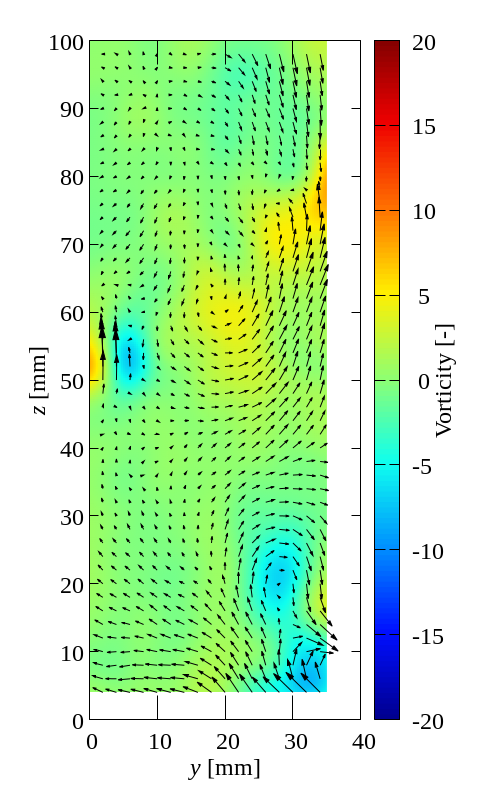
\includegraphics[keepaspectratio, width=44mm]{../images/Stop/time-averaged_vectors/velocity_and_vorticity.png}
      \subcaption{Without rotating tyre}
    \end{minipage} &
    \begin{minipage}[t]{0.45\hsize}
      \centering
      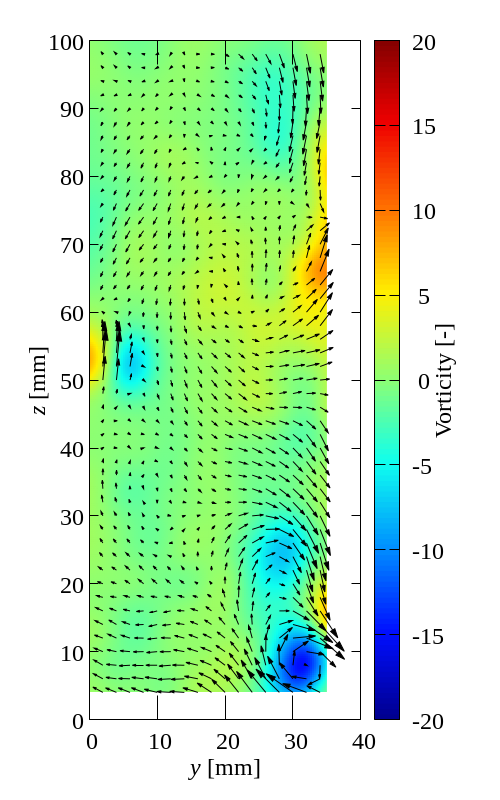
\includegraphics[keepaspectratio, width=44mm]{../images/Rotation_g=2mm/time-averaged_vectors/velocity_and_vorticity.png}
      \subcaption{With rotating tyre}
    \end{minipage}
  \end{tabular}
  \caption{Vehicle model}
\end{figure}

\newpage
\subsection{ガウシアンフィルタの標準偏差$\sigma$の検討}
クラスタ追跡によって取得したベクトル場を
2mm単位の格子点上に再配置する際,格子点まわりのベクトルを用いて推定する.
その際,任意に設定された標準偏差$\sigma$を持つガウス分布にしたがって重みづけを行うが,
$\sigma$の大きさによって解析できる鮮明度が変化する.
そこで,車両モデル(回転あり)の撮影結果を用いて,$\sigma$の違いによる変化を確認する.
以下のFig.2に示すのは,$\sigma$を変更し再配置を行った結果である.
結果より,$\sigma$が大きくなるにつれて,速度ベクトルは滑らかなつながりをみせ,
渦度の変化も小さくなっていることがわかる.

\begin{figure}[htbp]
  \centering
  \begin{tabular}{cc}
    \begin{minipage}[t]{0.45\hsize}
      \centering
      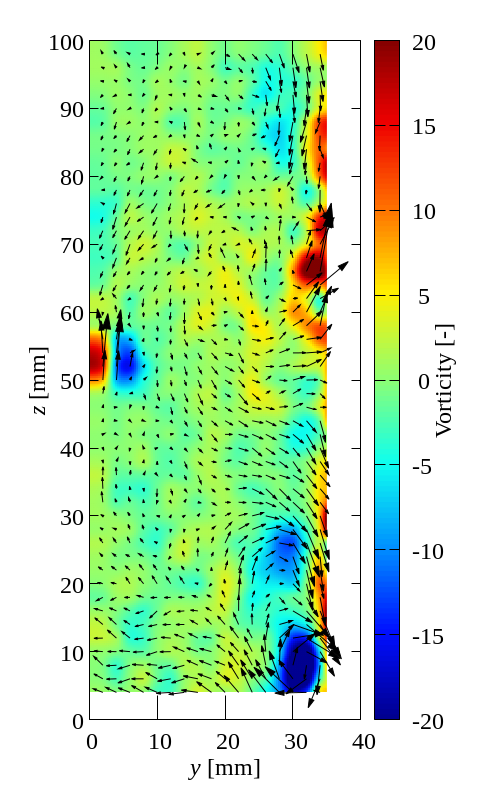
\includegraphics[keepaspectratio, width=44mm]{../images/Rotation_g=1mm/time-averaged_vectors/velocity_and_vorticity.png}
      \subcaption{$\sigma = 1$ [mm]}
    \end{minipage} &
    \begin{minipage}[t]{0.45\hsize}
      \centering
      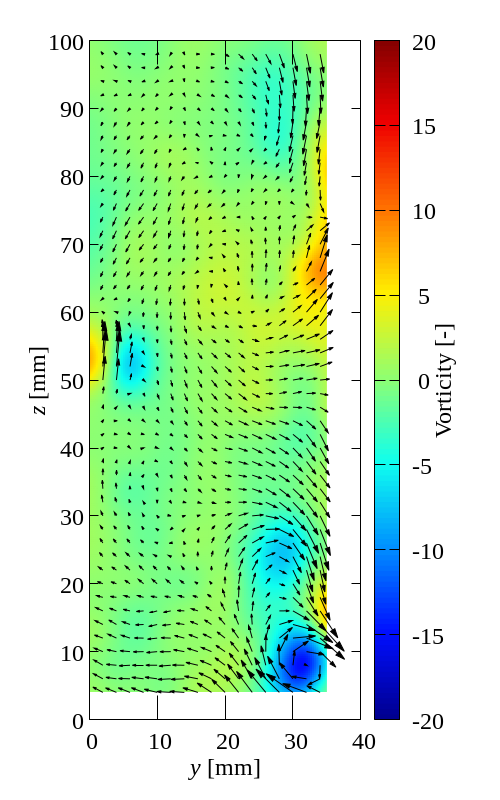
\includegraphics[keepaspectratio, width=44mm]{../images/Rotation_g=2mm/time-averaged_vectors/velocity_and_vorticity.png}
      \subcaption{$\sigma = 2$ [mm]}
    \end{minipage}
  \end{tabular}
  \begin{tabular}{cc}
    \begin{minipage}[t]{0.45\hsize}
      \centering
      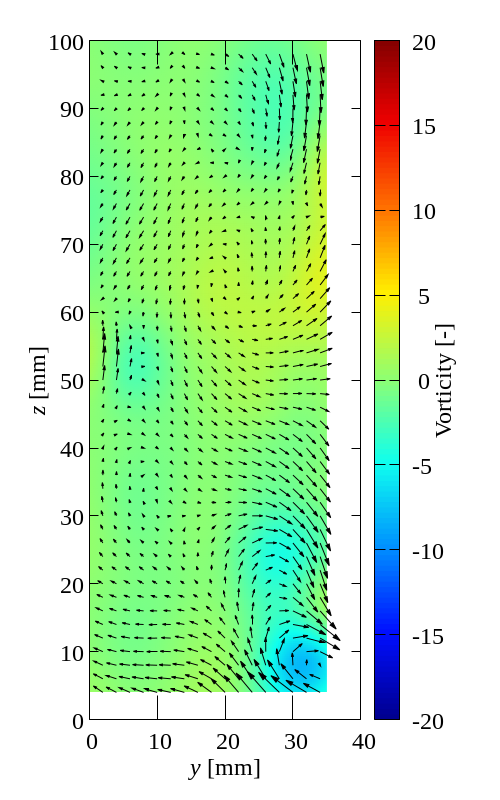
\includegraphics[keepaspectratio, width=44mm]{../images/Rotation_g=3mm/time-averaged_vectors/velocity_and_vorticity.png}
      \subcaption{$\sigma = 3$ [mm]}
    \end{minipage} &
    \begin{minipage}[t]{0.45\hsize}
      \centering
      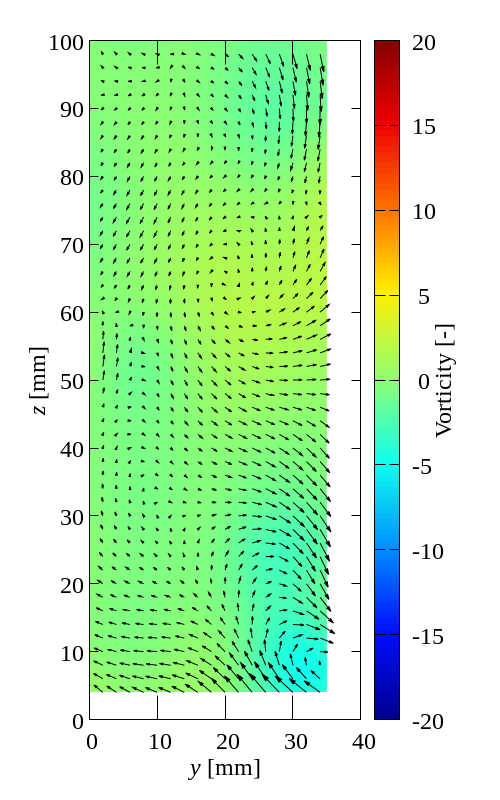
\includegraphics[keepaspectratio, width=44mm]{../images/Rotation_g=4mm/time-averaged_vectors/velocity_and_vorticity.png}
      \subcaption{$\sigma = 4$ [mm]}
    \end{minipage}
  \end{tabular}
  \caption{Particle Timeline}
\end{figure}

\newpage
\section{三角翼まわりの流れ場の測定}
解析アルゴリズムを用いた基礎実験として,
三角翼モデルの流れ場の撮影を再度行った.
今回は,翼の後端を $x = 0$ mm として,
10mm 刻みで $x = 100$ mm までの
計11ケースについて計測を行った.

\begin{table}[hbtp]
  \centering
  \caption{Condition of capturing images}
  \begin{tabular}{l c c}
    \hline
    Image size      & 800 $\times$ 600 & pixel \\ \hline
    Frame rate      & 800              & fps   \\ \hline
    Shutter speed   & 1/1000           & s     \\ \hline
    Capturing  time & 5.5              & s     \\ \hline
    Gain            & +7               & -     \\ \hline
  \end{tabular}
\end{table}

\begin{figure}[htbp]
  \centering
  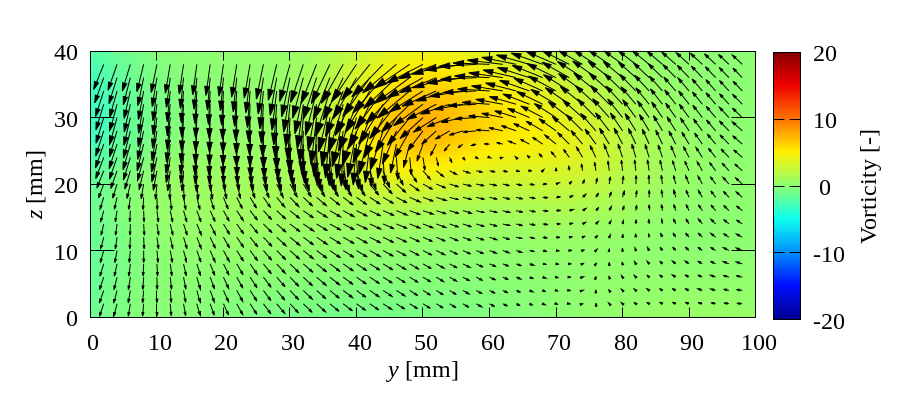
\includegraphics[keepaspectratio, width=85mm]{../images/Delta_x=0/time-averaged_vectors/velocity_and_vorticity.png}
  \caption{Wake of Delta Wing : x = 0}
  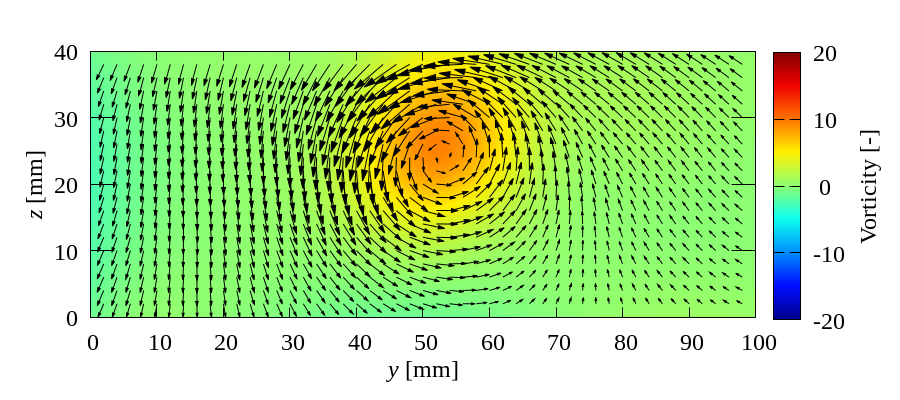
\includegraphics[keepaspectratio, width=85mm]{../images/Delta_x=50/time-averaged_vectors/velocity_and_vorticity.png}
  \caption{Wake of Delta Wing : x = 50}
  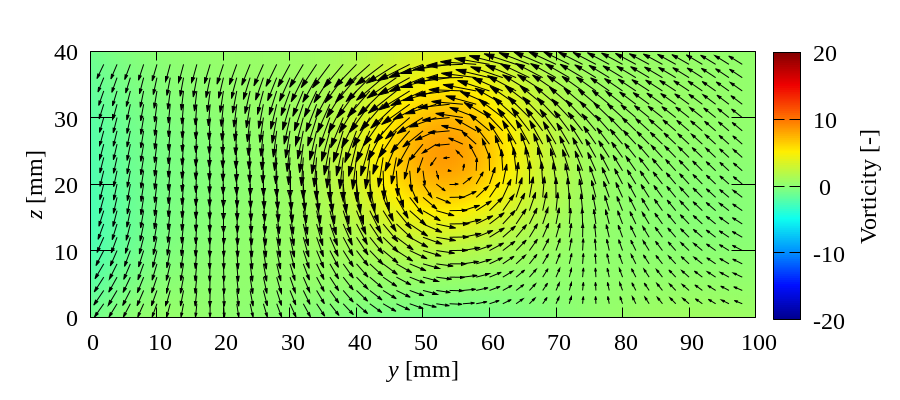
\includegraphics[keepaspectratio, width=85mm]{../images/Delta_x=100/time-averaged_vectors/velocity_and_vorticity.png}
  \caption{Wake of Delta Wing : x = 100}
\end{figure}


\newpage
\section{数値シミュレーションモデルの作成}
解析アルゴリズムの検証のため,
数値解析結果を用いた撮影画像シミュレーションの作成を行っている.\\
$\blacksquare$ \textgt{主な評価項目}
\begin{itemize}
  \item 粒子数密度
  \item レーザーシート間隔
\end{itemize}

\begin{figure}[htbp]
  \centering
  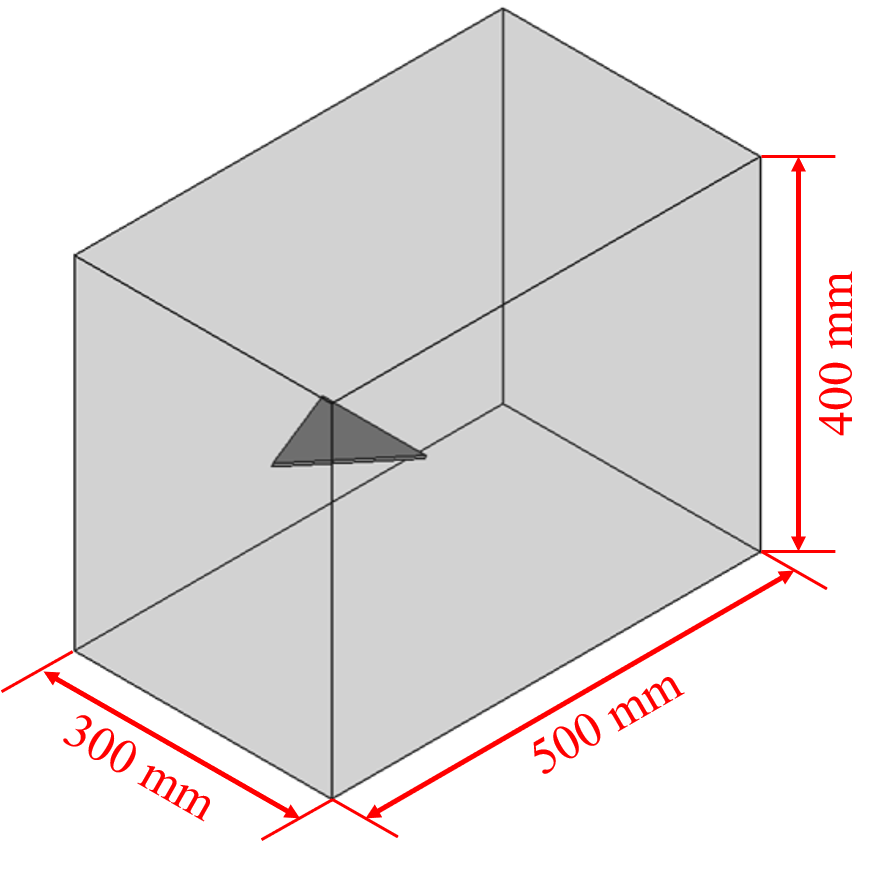
\includegraphics[keepaspectratio, width=55mm]{../images/model_3d.png}
  \caption{Simulation model : 3D}
  \vskip \baselineskip
  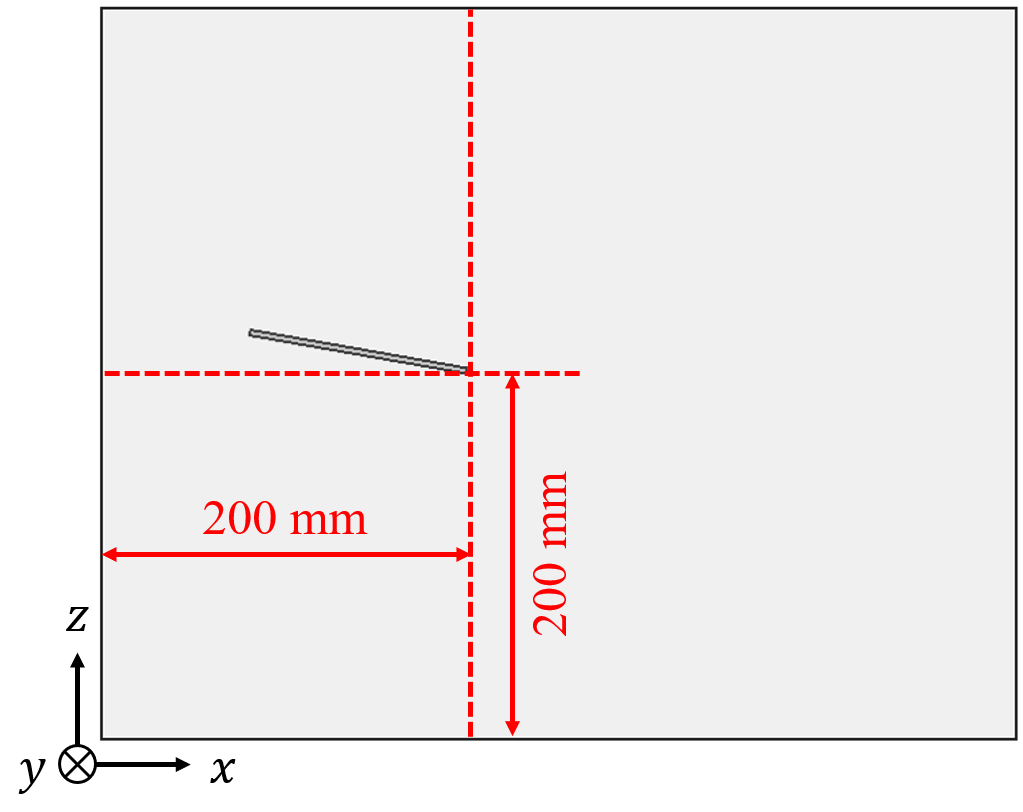
\includegraphics[keepaspectratio, width=55mm]{../images/model_xz_ver2.png}
  \caption{Simulation model : xz}
  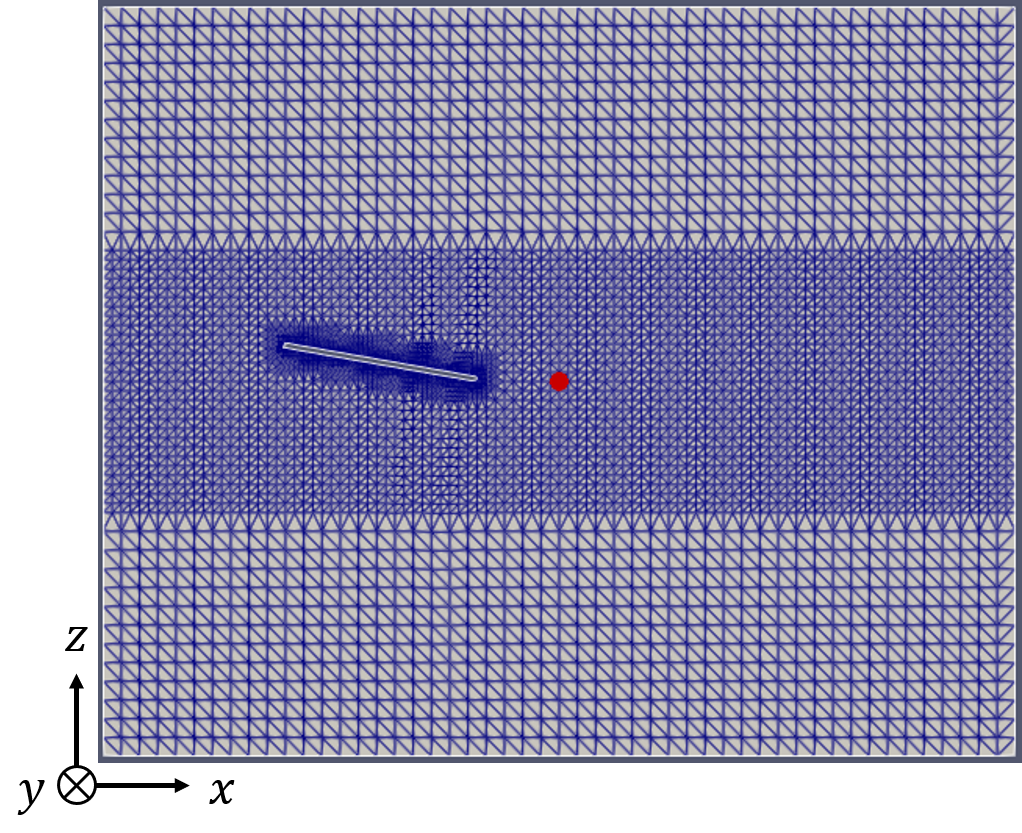
\includegraphics[keepaspectratio, width=55mm]{../images/Mesh_xz.png}
  \caption{Mesh of delta wing model}
\end{figure}


\section{来週の予定}
\begin{itemize}
  \item 数値シミュレーションデータの作成
  \item 三角翼モデル測定データの解析
  \item 車両モデルの測定
\end{itemize}

\end{document}